% This is samplepaper.tex, a sample chapter demonstrating the
% LLNCS macro package for Springer Computer Science proceedings;
% Version 2.20 of 2017/10/04
%
\documentclass[runningheads]{llncs}
%
\usepackage{graphicx}
\usepackage{amsmath}
\usepackage{amsfonts}
\usepackage{float}
% Used for displaying a sample figure. If possible, figure files should
% be included in EPS format.
%
% If you use the hyperref package, please uncomment the following line
% to display URLs in blue roman font according to Springer's eBook style:
% \renewcommand\UrlFont{\color{blue}\rmfamily}

\begin{document}
%
\title{Comparative approach between Krawtchouk moments and DCT-based dual watermarking for handwritten document images}
%
%\titlerunning{Abbreviated paper title}
% If the paper title is too long for the running head, you can set
% an abbreviated paper title here
%
\author{Ernesto Avila-Domenech\inst{1}\orcidID{0000-0002-4797-289X} \and
Alberto Taboada-Crispi\inst{2}\orcidID{0000-0002-7797-1441}}
%
\authorrunning{E. Avila-Domenech and A. Taboada-Crispi.}
% First names are abbreviated in the running head.
% If there are more than two authors, 'et al.' is used.
%
\institute{Universidad de Granma, Carretera Central v{\'i}a Holgu{\'i}n Km $\frac{1}{2}$, Granma, Cuba \email{\{eadomenech, asorial1983\}@gmail.com}\\ \and
	Universidad Central de Las Villas, Villa Clara, Cuba\\
	\email{\{ataboada\}@uclv.edu.cu}}
%
\maketitle              % typeset the header of the contribution
%
\begin{abstract}
The abstract should briefly summarize the contents of the paper in
150--250 words. Digital image watermarking is a powerful tool to secure digital image. In the present work, two dual digital image watermarking techniques based on Krawtchouk moments and Discrete Cosine Transform have been elaborated and compared. The comparative study is based on the values of the PSNR and BER.

\keywords{Digital Watermarking  \and Discrete Cosine Transform \and Krawtchouk moments.}
\end{abstract}
%
%
%
\section{Introduction}
Los documentos manuscritos atesorados en archivos historicos, bibliotecas y museos, constituyen una importante fuente de conocimiento e investigación para los historiadores y el público en general. Muchos de estos manuscritos están siendo digitalizados con el objetivo de preservar su integridad física y proveer acceso a una mayor cantidad de persona.

En el proceso de digitalizacion, es importante tener en cuenta la seguridad, pues pueden ser modificados y ser adjudicados a personas de manera ilícita.

Watermarking schemes can be divided into various categories. According to working domain, there are two types of watermarking scheme, spatial domain and frequency domain. The frequency domain schemes are generally considered more robust than the spatial domain schemes; this schemes consist in to transform an image from spatial domain to frequency domain. Some authors have made proposals based on Discrete Cosine Transform (DCT) \cite{munoz2018robust,wang2018blind}, this is because it has good energy compaction property that is widely used in image compression. Others have been based on Krawtchouk moments \cite{liu2017fractional,papakostas2014moment,Yap2004}.

On the other hand, for watermark insert process, various techniques are introduced and applied to watermarking schemes such as Spread Spectrum [3], Singular Value Decomposition (SVD) [9, 10, 11, 12, 13, 14] and Quantization Index Modulation (QIM) [5, 6, 7, 8, 14].

In this work, two dual digital image watermarking techniques based on Krawtchouk moments and Discrete Cosine Transform have been elaborated and compared. Both schemes used Dither Modulation Quantization (QIM-DM) and are optimized for handwritten document images. 

The rest of the paper is organized as follow; Section 2 summarize a preliminaries. Section 3 describes the proposed methods including robust watermarking and fragile watermarking. Experimental results are given in Section 4 and Section 5 concludes the paper.

\section{Preliminaries}
\subsection{Arnold transform}
The Arnold transform is a invertible method that can be used for pixel scrambling, and has been adopted in various watermarking schemes. By using the Arnold transform, the high pixel correlation can be disrupted. The Arnold transform is shown in Eq.~\ref{Arnold}, where $p$ and $q$ are positive integers, $det(A) = 1$, and $(x', y')$ are the new coordinates of the pixel after Arnold transform is applied to a pixel at position $(x, y)$ \cite{Chow2017}.
\begin{equation}
\left[\begin{array}{c}x'\\y'\end{array}\right]=A\left[\begin{array}{c}x\\y\end{array}\right]\ mod\ N=\left[\begin{array}{cc}1 & p\\q & pq+1\end{array}\right]\left[\begin{array}{c}x\\y\end{array}\right]\ mod\ N.
\label{Arnold}
\end{equation}

\subsection{Dither modulation quantization}
Dither modulation is an extension of traditional QIM algorithm proposed in \cite{chen2001quantization}. It has good performance on following requirements of watermarking: perceptibility ratio, data payload, robustness, and blind extraction. The combination of dither modulation quantization with different transformation domain watermarking methods also improves watermark extraction capability. The scheme has been applied successfully in watermarking algorithms \cite{avila2018watermarking,deng2009local,papakostas2014moment,zhu2016optimal}.

One bit of the watermark can be embedded as
\begin{equation}
|C{}_{0}^{'}(k_{1},k_{2})|=\begin{cases}
2\Delta\times round(\frac{|C{}_{0}(k_{1},k_{2})|}{2\Delta})+\frac{\Delta}{2}, & if\:W(i,j)=1\\
2\Delta\times round(\frac{|C{}_{0}(k_{1},k_{2})|}{2\Delta})-\frac{\Delta}{2} & if\:W(i,j)=0
\end{cases},
\label{DMEm}
\end{equation}
where $\Delta$ is the quantization step controlling the embedding strength of the watermark bit, $|\cdot|$ is the absolute operator, $round(\cdot)$ denotes the rounding operation to the nearest integer, $W(i,j)$ is the watermark bit at the position $(i,j)$ and $C{}_{0}^{'}(k_{1},k_{2})$ is the modified block. In general, a smaller $\Delta$ results in less visibility and poorer robustness while a larger $\Delta$ leads to higher visibility and better robustness.

To extract the watermark it is used
\begin{equation}
W^{*}(i,j)=arg_{\sigma\in\{0,1\}}min(|C_{0}^{''}(k_{1},k_{2})|_{\sigma}-|C_{0}^{*}(k_{1},k_{2})|)
\label{DMEx},
\end{equation}
where $W^{*}(i,j)$ is the extracted watermark, $C_{0}^{*}(k_{1},k_{2})$ the element $(k_1, k_2)$ of modified block and $|C_{0}^{''}(k_{1},k_{2})|_{\sigma}$ is defined as
\begin{equation}
|C_{0}^{''}(k_{1},k_{2})|_{\sigma}=\begin{cases}
2\Delta\times round(\frac{|C_{0}^{*}(k_{1},k_{2})|}{2\Delta})+\frac{\Delta}{2}, & if\:\sigma=1\\
2\Delta\times round(\frac{|C_{0}^{*}(k_{1},k_{2})|}{2\Delta})-\frac{\Delta}{2} & if\:\sigma=0
\end{cases}.
\end{equation}

\subsection{Krawtchouk moments}
The Krawtchouk moments were introduced by Yap in \cite{Yap2003}. These orthogonal moments satisfy the following recurrence relation
\begin{multline*}
\alpha_n(Np-2np+n-x)\overline{K}_{n}^{p,N}(x) \\= p(n-N)\overline{K}_{n+1}^{p,N}(x)+\beta_n n(1-p)\overline{K}_{n-1}^{p,N}(x),\quad n\geq 1,
\end{multline*}
with initial conditions 
\begin{equation*}
\overline{K}_{0}^{p,N}(x) = \sqrt{w^{p,N}(x)p^{-1}},
\end{equation*}	
and
\begin{equation*}
\overline{K}_{1}^{p,N}(x) = (Np-x)(Np)^{-1}\sqrt{w^{p,N}(x)(1-p)(Np)^{-1}},
\end{equation*}
where $\alpha_n = \sqrt{\frac{(1-p)(n+1)}{p(N-n)}}$, $\beta_n = \sqrt{\frac{(1-p)^2(n+1)n}{p^2(N-n)_2}}$, $w^{p,N}(x) = \binom{N}{x}p^x(1-p)^{N-x}$ and $0<p<1$.

The Krawtchouk moment of order $(m+n)$ of an image $f(x,y)$ with $M\times N$ pixels is defined as

\begin{equation}
K_{mn}=\sum_{x=0}^{M-1}\sum_{y=0}^{N-1}f(x,y)\overline{K}_{m}^{p,M}(x)\overline{K}_{n}^{q,N}(y),
\label{DKT}
\end{equation}
where $m\in \left[ 0,M-1\right] $ and $n\in \left[ 0,N-1\right] $.

The image $f(x,y)$ can be reconstructed using
\begin{equation}
f(x,y)=\sum_{m=0}^{M-1}\sum_{n=0}^{N-1}K_{mn}\overline{K}_{m}^{p,M}(x)\overline{K}_{n}^{q,N}(y),
\label{IDKT}
\end{equation}
where $x\in \left[ 0,M-1\right] $ and $y\in \left[ 0,N-1\right] $.

The lower order Krawtchouk moments store information of a specific region-of-interest of an image, the higher order moments store information of the rest of the image. Therefore, by reconstructing the image from the lower order moments and discarding the higher order moments, a sub-image can be extracted from the subject image. For each additional moment used in reconstructing the image, the square error of the reconstructed image is reduced \cite{Yap2003}.

The set of lower order Krawtchouk moments is generally the set of perceptually significant components of the image. This choice ensures that the watermark is robust to attacks \cite{Yap2004}.

\subsection{Discrete Cosine Transform (DCT)}
The DCT \cite{ahmed1974discrete} is a transform based on the Discrete Fourier Transform (DFT), but using only real numbers. Generally it is not applied to the image directly, but first that image is divided into blocks and then the transformation is applied to each block, resulting in a matrix divided into bands of low, medium and high frequencies. For an image of size $N\times N$ the equations used to calculate the DCT and its inverse (IDCT) are the following: 

\begin{equation}
D(u,v)=b(u)b(v)\sum_{x=0}^{N-1}\sum_{y=0}^{N-1}f(x,y)\cos\left[\frac{\left(2x+1\right)u\pi}{2N}\right]\cos\left[\frac{\left(2y+1\right)v\pi}{2N}\right]
\end{equation}

\begin{equation}
f(x,y)=\sum_{x=0}^{N-1}\sum_{y=0}^{N-1}b(u)b(v)D(u,v)\cos\left[\frac{\left(2x+1\right)u\pi}{2N}\right]\cos\left[\frac{\left(2y+1\right)v\pi}{2N}\right]
\end{equation}
where $D$ represents the coefficients of the DCT of the image and $f$ represents the function obtained when applying the IDCT. It is also defined that: 

\begin{equation}
b(u)=\begin{cases}
\frac{1}{\sqrt{N}} & ,u=0\\
\sqrt{\frac{2}{N}} & ,1\leq u\leq N-1
\end{cases}
\end{equation}

\begin{equation}
b(v)=\begin{cases}
\frac{1}{\sqrt{N}} & ,v=0\\
\sqrt{\frac{2}{N}} & ,1\leq v\leq N-1
\end{cases}
\end{equation}

The first coefficient of the matrix obtained when applying the DCT to a block (DC coefficient) is simply the average of the remaining coefficients of the block. The remaining coefficients represent successively increasing frequencies.

\section{Dual watermarking techniques}
Dual watermarking implies embedding of fragile as well as robust watermarks into the same cover image. It facilitates integration of image authentication and copyright protection into the same scheme. First robust watermarking and then the fragile watermarking should be done because the fragile watermarking is sensitive to small changes. Unlike the fragile watermarking, the robust one resists changes caused by performing the fragile watermarking.

The robust watermarking method proposed is similar to the one proposed in \cite{avila2018watermarking}. The difference consists of considering any binary image as a watermark. In the previous work only a QR code was considered as a watermark, so it was possible a restructuring of the extracted watermark making use of the characteristics related to the QR codes.
\begin{figure}
	\begin{center}
		\includegraphics[width=\textwidth]{WP.png}
	\end{center}
	\caption{Watermark embedding and extraction scheme. (Modified from \cite{avila2018watermarking})}
	\label{PIE}
\end{figure}

The following steps are taken during the embedding process:
\begin{enumerate}
	\item The binary watermark image is scrambled using Arnold Transform (see Eq.~\ref{Arnold}).
	\item The cover image is transformed from RGB to YCbCr color space, and the Y component, corresponding to the luminance information, is divided into small image blocks of $8\times 8$ pixels.
	\item A number of blocks equal to the number of bits to be inserted is selected from a given key.
	\item The Krawtchouk moments \cite{Yap2003} of the selected blocks are determined.
	\item Watermark bit is embedded in the selected block moments using Dither modulation \cite{chen2001quantization}. The values 19 and 128 are used as the coefficient and embedding strength values respectively. Watermarked blocks can be obtained. 
	\item The YCbCr to RGB color space is transformed to obtain RGB watermarked image.
\end{enumerate}

For watermark extraction:
\begin{enumerate}
	\item The watermarked image is transformed from the RGB to the YCbCr color space and the Y component is divided into $8\times 8$ pixels blocks.
	\item Some blocks are selected from which they will be extracted from the key used in the embedding process.
	\item The Krawtchouk moments of the selected blocks are determined.
	\item Scrambled watermark bits are obtained with the selected blocks moments using Dither modulations.
	\item Finally, a watermark is constructed with the scrambled bits using Arnold transform.
\end{enumerate}

For the process of embedding the fragile watermark for tampered small changes, the following steps are performed each RGB component:
\begin{enumerate}
	\item The component is divided into $32\times 32$ non-overlapped blocks.
	\item 128 pixels of each block are selected by a given key.
	\item The least significant bit (LSB) of each selected pixel is assigned the value 0.
	\item The MD5 hash value of the modified block is generated as a watermark.
	\item The watermark is embedded into the LSB of the selected pixels and a watermarked block image is obtained.  
\end{enumerate}    

Detecting a fragile watermark is the reverse process of embedding watermark, which is used to detect whether the watermarked image has been tampered and what the precise position of the tampered parts is. For this:
\begin{enumerate}
	\item The RGB image is divided into $32\times 32$ non-overlapped blocks.
	\item 128 pixels of each block are selected by a given key.
	\item Three binary series are formed from the LSBs of the selected pixels.
	\item The LSBs of each selected pixel are assigned the value 0.
	\item The MD5 hash value of the modified block is generated and compared with obtained series.
\end{enumerate}

\subsection{Krawtchouk moments-based dual watermarking}
The $p$ and $q$ parameters used in Eq.~\ref{DKT} and Eq.~\ref{IDKT} are the parameters of the Krawtchouk polynomials that control their locality behaviour, that define the specific host areas control the horizontal and vertical direction of the watermark localization, respectively. In this work, it was taken $p=q=0.7$.
\begin{figure} [H]
	\begin{center}
		\includegraphics[width=\textwidth]{colormapDKT.eps}
	\end{center}
	\caption{Colormap}
	\label{colormapDKT}
\end{figure}

\subsection{DCT-based dual watermarking}
\begin{figure} [H]
	\begin{center}
		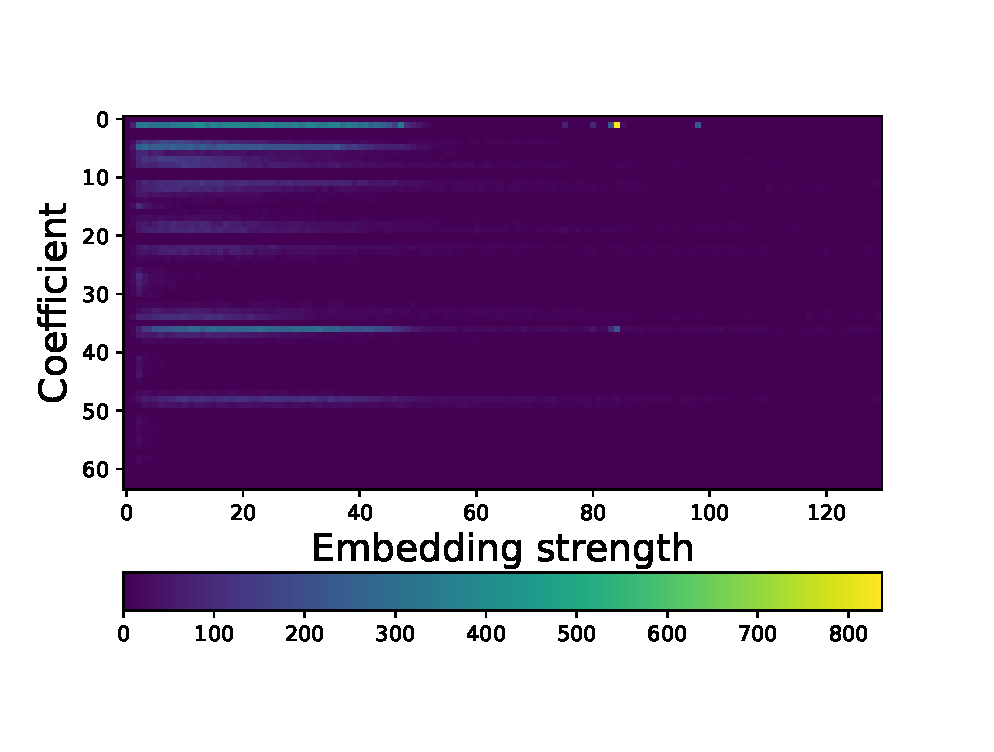
\includegraphics[width=\textwidth]{colormapDCT.eps}
	\end{center}
	\caption{Colormap}
	\label{colormapDCT}
\end{figure}

\section{Experiments and Results}
We used two handwriten document image databases: Saint Gall \cite{fischer2011transcription} and Parzival \cite{fischer2009automatic} database. The first one contains manuscripts from the 9th century using Carolingian scripts by a single writer, while the Parzival is compiled from 13th century Gothic scripts \cite{pastor2016complete}.

\subsection{Imperceptibility}
We calculated the larger peak signal-to-noise ratio (PSNR) which compares the similarity between the original image $ I $, and the watermarked image $ I_w $. A higher PSNR indicates that the watermarked image more closely resembles the original image meaning that the watermark is more imperceptible.
\begin{figure}[H]
	\begin{center}
		\begin{tabular}{|c|c|}\hline
			\includegraphics[width=0.5\textwidth]{PSNR_saintgall.eps}
			&\includegraphics[width=0.5\textwidth]{PSNR_parzival.eps}\\\hline
		\end{tabular}
	\end{center}
	\caption{PSNR values for Saint Gall and Parzival database watermarked images.}
	\label{psnr}
\end{figure}

\begin{figure}
	\begin{center}
		\begin{tabular}{|c|c|}\hline
			\includegraphics[width=0.5\textwidth]{PSNRwsizeSaintGall.eps}
			&\includegraphics[width=0.5\textwidth]{PSNRwsizeParzival.eps}\\\hline
		\end{tabular}
	\end{center}
	\caption{PSNR behavior to mark the ``csg562-003.jpg'' image of Saint Gall database and ``d-006.jpg'' image of Perzival database with watermarks of different sizes.}
	\label{psnrwsize}
\end{figure}

\subsection{Robustness}
The robustness is measured as the bit error rate (BER) corresponding to incorrectly formed binary values of the watermark image.
\begin{figure}[H]
	\begin{center}
		\begin{tabular}{|c|c|}\hline
			\includegraphics[width=0.5\textwidth]{BER75SaintGall.eps}
			&\includegraphics[width=0.5\textwidth]{BER75Parzival.eps}\\\hline
		\end{tabular}
	\end{center}
	\caption{BER values for watermarked images with JPEG compression (QF=75\%).}
	\label{ber75}
\end{figure}

The main contributions of this paper are of twofold. First is the obtaining of better values of imperceptibility, and the second is the remarkable improvement in the strength when JPEG compression attacks at 75\%, 50\% and 25\% are applied (see Figs. \ref{ber75}-\ref{ber25}). Similar to the PSNR, a preliminary experiment, using the same two images, was performed to obtain the corresponding BER by varying the size of the watermark.
\begin{figure}[H]
	\begin{center}
		\begin{tabular}{|c|c|}\hline
			\includegraphics[width=0.5\textwidth]{BER50SaintGall.eps}
			&\includegraphics[width=0.5\textwidth]{BER50Parzival.eps}\\\hline
		\end{tabular}
	\end{center}
	\caption{BER values for watermarked images with JPEG compression (QF=50\%).}
	\label{ber50}
\end{figure}
\begin{figure}[H]
	\begin{center}
		\begin{tabular}{|c|c|}\hline
			\includegraphics[width=0.5\textwidth]{BER25SaintGall.eps}
			&\includegraphics[width=0.5\textwidth]{BER25Parzival.eps}\\\hline
		\end{tabular}
	\end{center}
	\caption{BER values for watermarked images with JPEG compression (QF=25\%).}
	\label{ber25}
\end{figure} 

\begin{figure}
	\begin{center}
		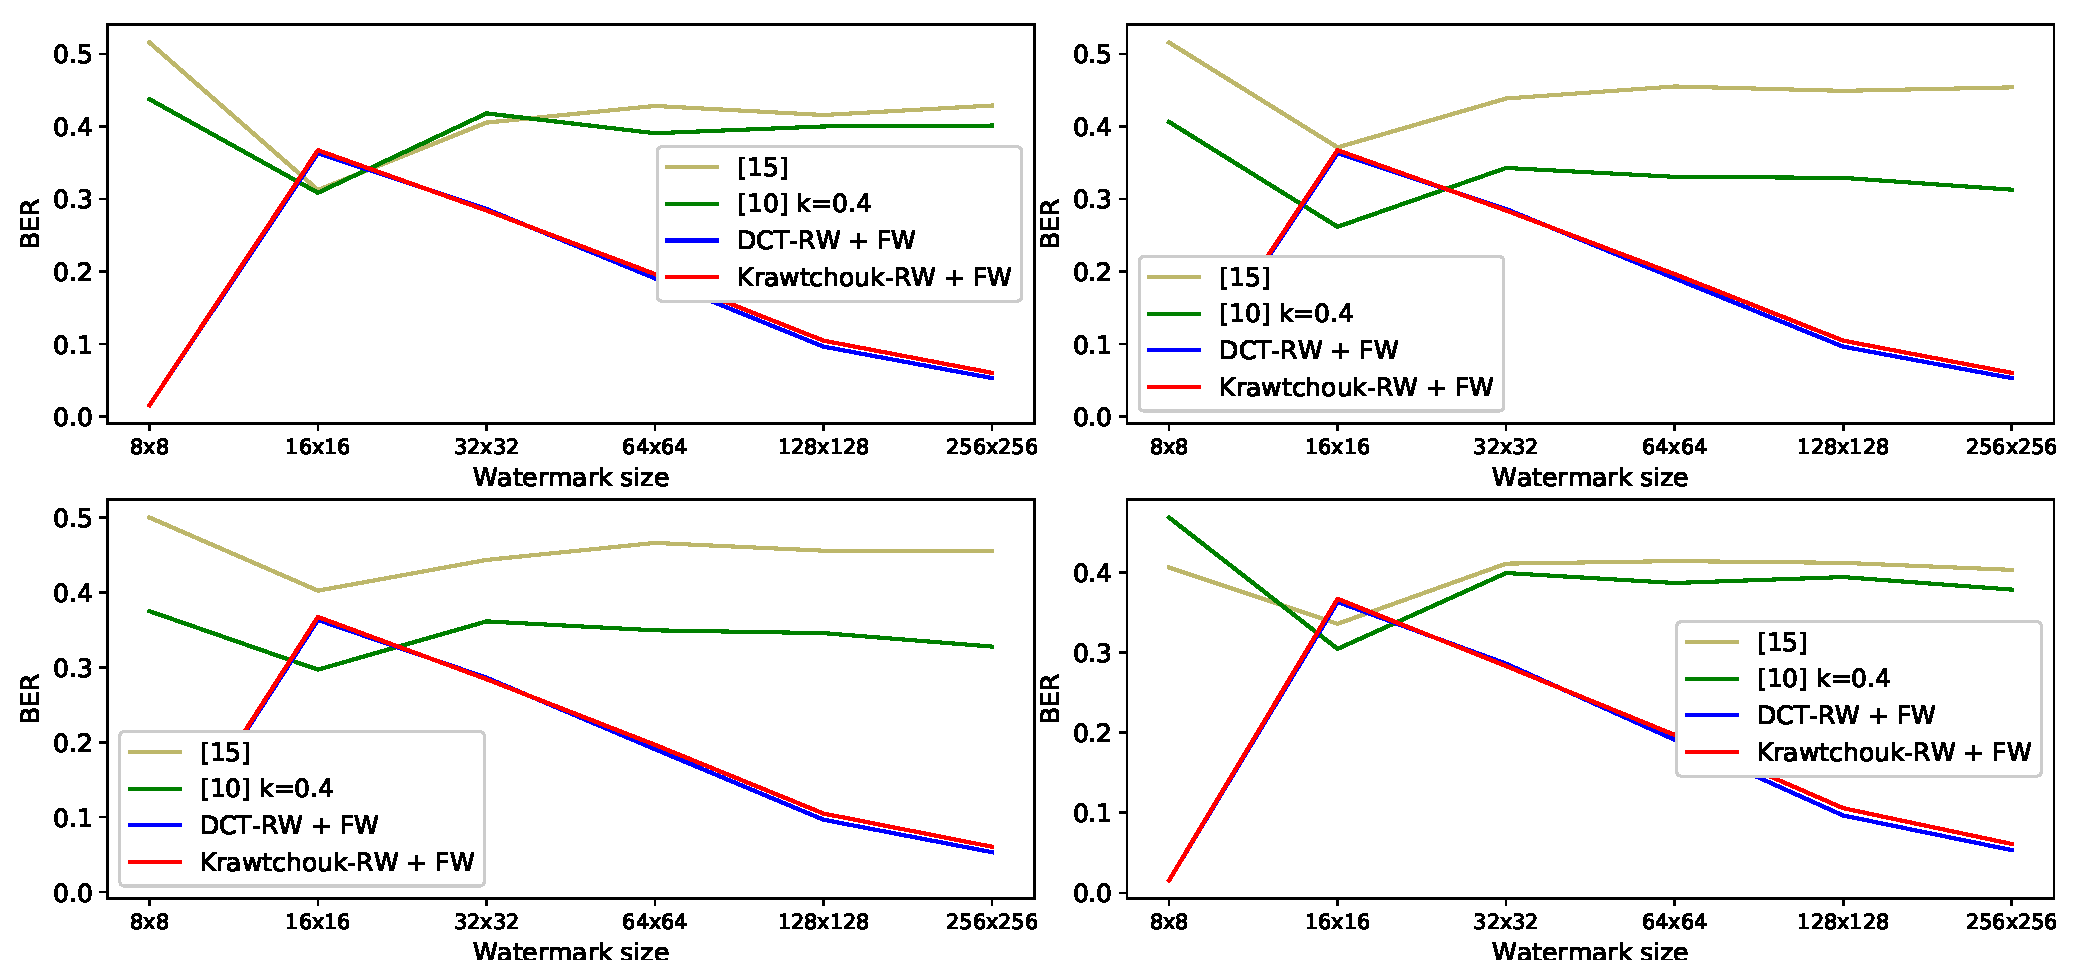
\includegraphics[width=1.1\textwidth]{BERwsizeSaintGall.eps}
		\caption{BER behavior to mark the image ``csg562-003.jpg'' of Saint Gall database with watermarks of different sizes when no attack is applied, a JPEG compression is performed with QF = 75\%, 50\% and 25\% respectively.} \label{berwsizeSaintGall}
	\end{center}
\end{figure}

\begin{figure}
	\begin{center}
		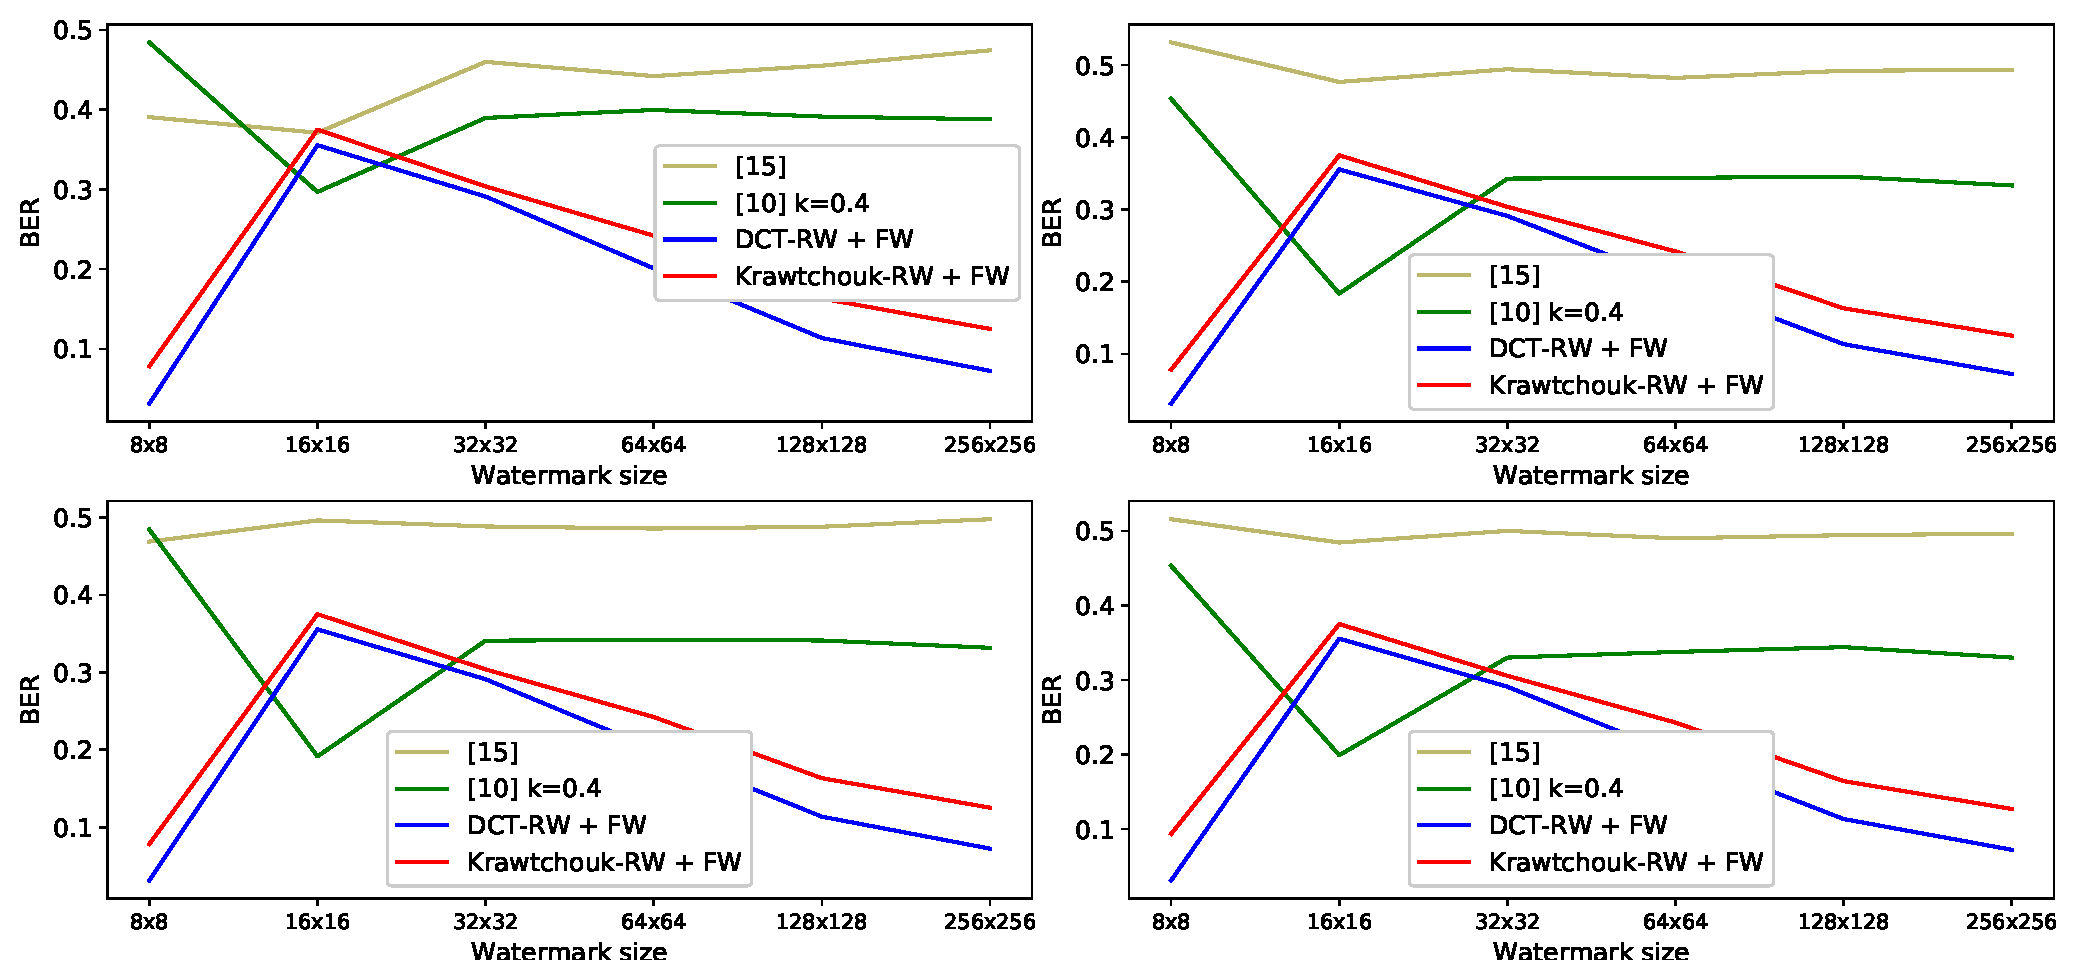
\includegraphics[width=1.1\textwidth]{BERwsizeParzival.eps}
		\caption{BER behavior to mark the image ``d-006.jpg'' of the Parzival database with watermarks of different sizes when no attack is applied, a JPEG compression is performed with QF = 75\%, 50\% and 25\% respectively.} \label{berwsizeParzival}
	\end{center}
\end{figure}

\section{Conclusions}
This work provides an innovative image watermarking scheme in two transform domains Krawtchouk moments and DCT. Both the domains are good enough.

% ---- Bibliography ----
%
% BibTeX users should specify bibliography style 'splncs04'.
% References will then be sorted and formatted in the correct style.
%
\bibliographystyle{splncs04}
\bibliography{mybibliography}
%
\end{document}